\section{Тестовые задачи}

\begin{frame}
\begin{center}
\frametitle{Тестовые задачи}
\framesubtitle{\ }
\end{center}
\end{frame}

\begin{frame}
\frametitle{Тестовые задачи}
\framesubtitle{Двумерная задача просачивания с источником на границе}
\begin{center}
Начальные условия: 
\begin{equation*}
  \begin{aligned}
    &T=285K,\ P_w=P_\text{атм},\ S_w=0.1,\\
    &S_n(x, y)=0.4 + 0.1 \cdot sin^2(x \cdot N_x + y \cdot N_y),\\
    &S_g(x, y)=0.4 + 0.1 \cdot cos^2(x \cdot N_x + y \cdot N_y).
   \end{aligned}
\end{equation*}
Граничные условия:
\begin{figure}
\begin{minipage}[h]{0.24\textwidth}
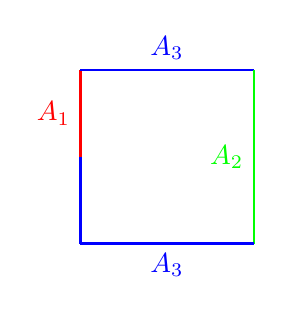
\begin{tikzpicture}
  \draw[blue,thick] (0,0) -- (0,1.1);
  \draw[red,thick] (0,1.1) -- node[anchor=east]{$A_1$}(0,2.2);
  \draw[blue,thick] (0,2.2) -- node[anchor=south]{$A_3$}(2.2,2.2);
  \draw[green,thick] (2.2,2.2) -- node[anchor=east]{$A_2$}(2.2,0);
  \draw[blue,thick] (2.2,0) -- node[anchor=north]{$A_3$}(0,0);
\end{tikzpicture}
\end{minipage}
\hfill
\begin{minipage}[h]{0.75\textwidth}
  \begin{tabular}{ l l l l }
    $A_1:\ T=320K,$ & $P_w=1.1\cdot P_{\text{атм}},$ & $S_w=0.6,$ & $S_n=0.15;$\\
      & & & \\
    $A_2:\ \dfrac{\partial{T}}{\partial{x}}=0,$ & ${P_w}=P_{\text{атм}},$ & $\dfrac{\partial{S_w}}{\partial{x}}=0,$ & $\dfrac{\partial{S_n}}{\partial{x}}=0;$\\
      & & & \\
    $A_3:\ \dfrac{\partial{T}}{\partial{x}}=0,$ & $\dfrac{\partial{P_w}}{\partial{x}}=0,$ & $\dfrac{\partial{S_w}}{\partial{x}}=0,$ & $\dfrac{\partial{S_n}}{\partial{x}}=0.$
  \end{tabular}
\end{minipage}
\end{figure}
\end{center}
\end{frame}


\begin{frame}
\frametitle{Тестовые задачи}
\framesubtitle{Двумерная задача просачивания с источником на границе}
\begin{center}
\begin{figure}
\begin{columns}[T]
\begin{column}{.33\textwidth}
\vspace*{-1.5mm}
\begin{tikzpicture}
  \begin{axis}[view={0}{90}, enlargelimits=false, colorbar left, colorbar style={width=0.2cm}, width=1.0\textwidth, height=1.0\textwidth, point meta min=100000, point meta max=110000]
    \pgfplotstableread[skip first n=3]{data/test3/F-000000000100.tec}{\mytable}
    \addplot3 [surf, shader=interp] table [x=0, y=1, z=5] {\mytable};
  \end{axis}
\end{tikzpicture}
\caption{$\qquad \qquad \qquad P_w,\ t=100$с}
\end{column}
\hspace{10mm}
\begin{column}{.33\textwidth}
\begin{tikzpicture}
  \begin{axis}[view={0}{90}, enlargelimits=false, width=1.0\textwidth, height=1.0\textwidth, point meta min=100000, point meta max=110000]
    \pgfplotstableread[skip first n=3]{data/test3/F-000000001000.tec}{\mytable}
    \addplot3 [surf, shader=interp] table [x=0, y=1, z=5] {\mytable};
  \end{axis}
\end{tikzpicture}
\caption{$P_w,\ t=1000$с}
\end{column}
\hfill
\begin{column}{.33\textwidth}
\begin{tikzpicture}
  \begin{axis}[view={0}{90}, enlargelimits=false, width=1.0\textwidth, height=1.0\textwidth, point meta min=100000, point meta max=110000]
    \pgfplotstableread[skip first n=3]{data/test3/F-000000007000.tec}{\mytable}
    \addplot3 [surf, shader=interp] table [x=0, y=1, z=5] {\mytable};
  \end{axis}
\end{tikzpicture}
\caption{$P_w,\ t=7000$с}
\end{column}
\end{columns}
\begin{columns}[T]
\begin{column}{.33\textwidth}
\begin{tikzpicture}
  \begin{axis}[view={0}{90}, enlargelimits=false, colorbar left, colorbar style={width=0.2cm}, width=1.0\textwidth, height=1.0\textwidth, point meta min=285, point meta max=320]
    \pgfplotstableread[skip first n=3]{data/test3/F-000000000100.tec}{\mytable}
    \addplot3 [surf, shader=interp] table [x=0, y=1, z=6] {\mytable};
  \end{axis}
\end{tikzpicture}
\caption{$\qquad \qquad \qquad T,\ t=100$с}
\end{column}
\hspace{10mm}
\begin{column}{.33\textwidth}
\begin{tikzpicture}
  \begin{axis}[view={0}{90}, enlargelimits=false, width=1.0\textwidth, height=1.0\textwidth, point meta min=285, point meta max=320]
    \pgfplotstableread[skip first n=3]{data/test3/F-000000001000.tec}{\mytable}
    \addplot3 [surf, shader=interp] table [x=0, y=1, z=6] {\mytable};
  \end{axis}
\end{tikzpicture}
\caption{$T,\ t=1000$с}
\end{column}
\hfill
\begin{column}{.33\textwidth}
\begin{tikzpicture}
  \begin{axis}[view={0}{90}, enlargelimits=false, width=1.0\textwidth, height=1.0\textwidth, point meta min=285, point meta max=320]
    \pgfplotstableread[skip first n=3]{data/test3/F-000000007000.tec}{\mytable}
    \addplot3 [surf, shader=interp] table [x=0, y=1, z=6] {\mytable};
  \end{axis}
\end{tikzpicture}
\caption{$T,\ t=7000$с}
\end{column}
\end{columns}
\end{figure}
\end{center}
\end{frame}


\begin{frame}
\frametitle{Тестовые задачи}
\framesubtitle{Двумерная задача просачивания с источником на границе}
\begin{center}
\begin{figure}
\begin{columns}[T]
\begin{column}{.33\textwidth}
\begin{tikzpicture}
  \begin{axis}[view={0}{90}, enlargelimits=false, colorbar left, colorbar style={width=0.2cm}, width=1.0\textwidth, height=1.0\textwidth, point meta min=0.1, point meta max=0.48]
    \pgfplotstableread[skip first n=3]{data/test3/F-000000000100.tec}{\mytable}
    \addplot3 [surf, shader=interp] table [x=0, y=1, z=2] {\mytable};
  \end{axis}
\end{tikzpicture}
\caption{$\qquad \qquad \qquad S_w,\ t=100$с}
\end{column}
\hspace{10mm}
\begin{column}{.33\textwidth}
\begin{tikzpicture}
  \begin{axis}[view={0}{90}, enlargelimits=false, width=1.0\textwidth, height=1.0\textwidth, point meta min=0.1, point meta max=0.48]
    \pgfplotstableread[skip first n=3]{data/test3/F-000000001000.tec}{\mytable}
    \addplot3 [surf, shader=interp] table [x=0, y=1, z=2] {\mytable};
  \end{axis}
\end{tikzpicture}
\caption{$S_w,\ t=1000$с}
\end{column}
\hfill
\begin{column}{.33\textwidth}
\begin{tikzpicture}
  \begin{axis}[view={0}{90}, enlargelimits=false, width=1.0\textwidth, height=1.0\textwidth, point meta min=0.1, point meta max=0.48]
    \pgfplotstableread[skip first n=3]{data/test3/F-000000007000.tec}{\mytable}
    \addplot3 [surf, shader=interp] table [x=0, y=1, z=2] {\mytable};
  \end{axis}
\end{tikzpicture}
\caption{$S_w,\ t=7000$с}
\end{column}
\end{columns}
\begin{columns}[T]
\begin{column}{.33\textwidth}
\begin{tikzpicture}
  \begin{axis}[view={0}{90}, enlargelimits=false, colorbar left, colorbar style={width=0.2cm}, width=1.0\textwidth, height=1.0\textwidth, point meta min=0.1, point meta max=0.48]
    \pgfplotstableread[skip first n=3]{data/test3/F-000000000100.tec}{\mytable}
    \addplot3 [surf, shader=interp] table [x=0, y=1, z=3] {\mytable};
  \end{axis}
\end{tikzpicture}
\caption{$\qquad \qquad \qquad S_n,\ t=100$с}
\end{column}
\hspace{10mm}
\begin{column}{.33\textwidth}
\begin{tikzpicture}
  \begin{axis}[view={0}{90}, enlargelimits=false, width=1.0\textwidth, height=1.0\textwidth, point meta min=0.1, point meta max=0.48]
    \pgfplotstableread[skip first n=3]{data/test3/F-000000001000.tec}{\mytable}
    \addplot3 [surf, shader=interp] table [x=0, y=1, z=3] {\mytable};
  \end{axis}
\end{tikzpicture}
\caption{$S_n,\ t=1000$с}
\end{column}
\hfill
\begin{column}{.33\textwidth}
\begin{tikzpicture}
  \begin{axis}[view={0}{90}, enlargelimits=false, width=1.0\textwidth, height=1.0\textwidth, point meta min=0.1, point meta max=0.48]
    \pgfplotstableread[skip first n=3]{data/test3/F-000000007000.tec}{\mytable}
    \addplot3 [surf, shader=interp] table [x=0, y=1, z=3] {\mytable};
  \end{axis}
\end{tikzpicture}
\caption{$S_n,\ t=7000$с}
\end{column}
\end{columns}
\end{figure}
\end{center}
\end{frame}


\begin{frame}
\frametitle{Тестовые задачи}
\framesubtitle{Двумерная задача просачивания с источником на границе}
\begin{center}
\begin{figure}
\begin{columns}[T]
\begin{column}{.33\textwidth}
\begin{tikzpicture}
  \begin{axis}[view={0}{90}, enlargelimits=false, colorbar left, colorbar style={width=0.2cm}, width=1.0\textwidth, height=1.0\textwidth, point meta min=0.1, point meta max=0.48]
    \pgfplotstableread[skip first n=3]{data/test3/F-000000000100.tec}{\mytable}
    \addplot3 [surf, shader=interp] table [x=0, y=1, z=4] {\mytable};
  \end{axis}
\end{tikzpicture}
\caption{$\qquad \qquad \qquad S_g,\ t=100$с}
\end{column}
\hspace{10mm}
\begin{column}{.33\textwidth}
\begin{tikzpicture}
  \begin{axis}[view={0}{90}, enlargelimits=false, width=1.0\textwidth, height=1.0\textwidth, point meta min=0.1, point meta max=0.48]
    \pgfplotstableread[skip first n=3]{data/test3/F-000000001000.tec}{\mytable}
    \addplot3 [surf, shader=interp] table [x=0, y=1, z=4] {\mytable};
  \end{axis}
\end{tikzpicture}
\caption{$S_g,\ t=1000$с}
\end{column}
\hfill
\begin{column}{.33\textwidth}
\begin{tikzpicture}
  \begin{axis}[view={0}{90}, enlargelimits=false, width=1.0\textwidth, height=1.0\textwidth, point meta min=0.1, point meta max=0.48]
    \pgfplotstableread[skip first n=3]{data/test3/F-000000007000.tec}{\mytable}
    \addplot3 [surf, shader=interp] table [x=0, y=1, z=4] {\mytable};
  \end{axis}
\end{tikzpicture}
\caption{$S_g,\ t=7000$с}
\end{column}
\end{columns}
\end{figure}
\end{center}
\end{frame}




\begin{frame}
\frametitle{Тестовые задачи}
\framesubtitle{Трехмерная задача просачивания в резервуаре с источником на границе}
\begin{center}
Начальные условия:
\begin{equation*}
  \begin{aligned}
    &P_w=P_\text{атм},\ T=285K,\ S_w=0.1,\\
    &S_n(x, y, z)=0.4 + 0.1 \cdot sin^2(x \cdot N_x + y \cdot N_y + z \cdot N_z),\\
    &S_g(x, y, z)=0.4 + 0.1 \cdot cos^2(x \cdot N_x + y \cdot N_y + z \cdot N_z).
   \end{aligned}
\end{equation*}

Граничные условия:

\newcommand{\Depth}{2}
\newcommand{\Height}{2}
\newcommand{\Width}{2}

\begin{figure}
\begin{minipage}[h]{0.24\textwidth}
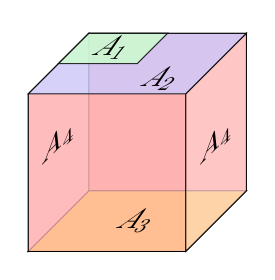
\begin{tikzpicture}
\coordinate (O) at (0,0,0);
\coordinate (A) at (0,\Width,0);
\coordinate (B) at (0,\Width,\Height);
\coordinate (C) at (0,0,\Height);
\coordinate (D) at (\Depth,0,0);
\coordinate (E) at (\Depth,\Width,0);
\coordinate (F) at (\Depth,\Width,\Height);
\coordinate (G) at (\Depth,0,\Height);

\coordinate (H) at (0, \Width, \Height/2);
\coordinate (I) at (\Depth/2, \Width,0);
\coordinate (J) at (\Depth/2, \Width, \Height/2);

\draw[black,fill=yellow!90] (O) -- (C) -- (G) -- (D) -- cycle;% Bottom Face
\draw[black,fill=red!30] (O) -- (A) -- (E) -- (D) -- cycle;% Back Face
\draw[black,fill=red!10] (O) -- (A) -- (B) -- (C) -- cycle;% Left Face
\draw[black,fill=red!20,opacity=0.8] (D) -- (E) -- (F) -- (G) -- cycle;% Right Face
\draw[black,fill=red!30,opacity=0.8] (C) -- (B) -- (F) -- (G) -- cycle;% Front Face
\draw[black,fill=blue!20,opacity=0.8] (A) -- (B) -- (F) -- (E) -- cycle;% Top Face

\draw[black,fill=green!20,opacity=0.8] (A) -- (H) -- (J) -- (I) -- cycle;% Top Face

\node[xslant=0.8] at (\Depth/4, \Width, \Height/4) {$A_1$};
\node[xslant=0.8] at (3*\Depth/4, \Width, 3*\Height/4) {$A_2$};
\node[xslant=0.8] at (\Depth/2, 0, \Height/2) {$A_3$};

\node[yslant=1.0] at (\Depth, \Width/2, \Height/2) {$A_4$};
\node[yslant=1.0] at (0, \Width/2, \Height/2) {$A_4$};
\end{tikzpicture}
\end{minipage}
\hfill
\begin{minipage}[h]{0.75\textwidth}
 \begin{equation*}
  \begin{aligned}
    &A_1:\ T=320K,\ S_w=0.6,\ S_n=0.05,\ P_i=P_{\text{атм}};\\
    &A_2:\ \dfrac{\partial{T}}{\partial{x}}=\dfrac{\partial{S_w}}{\partial{x}}=\dfrac{\partial{S_n}}{\partial{x}}=0,\ {P_i}=P_{\text{атм}};\\
    &A_3:\ \dfrac{\partial{T}}{\partial{x}}=\dfrac{\partial{S_w}}{\partial{x}}=\dfrac{\partial{S_n}}{\partial{x}}=0,\ P_i\leftarrow(\overrightarrow{u_i} \cdot \overrightarrow{n})=0;\\
    &A_4:\ \dfrac{\partial{T}}{\partial{x}}=\dfrac{\partial{S_w}}{\partial{x}}=\dfrac{\partial{S_n}}{\partial{x}}=0,\ \dfrac{\partial{P_i}}{\partial{x}}=0.
  \end{aligned}
 \end{equation*}
\end{minipage}
\end{figure}
\end{center}
\end{frame}


\begin{frame}
\frametitle{Тестовые задачи}
\framesubtitle{Трехмерная задача просачивания в резервуаре с источником на границе}
\begin{center}
\begin{figure}
  \movie[width=1.0\textwidth,showcontrols=false]{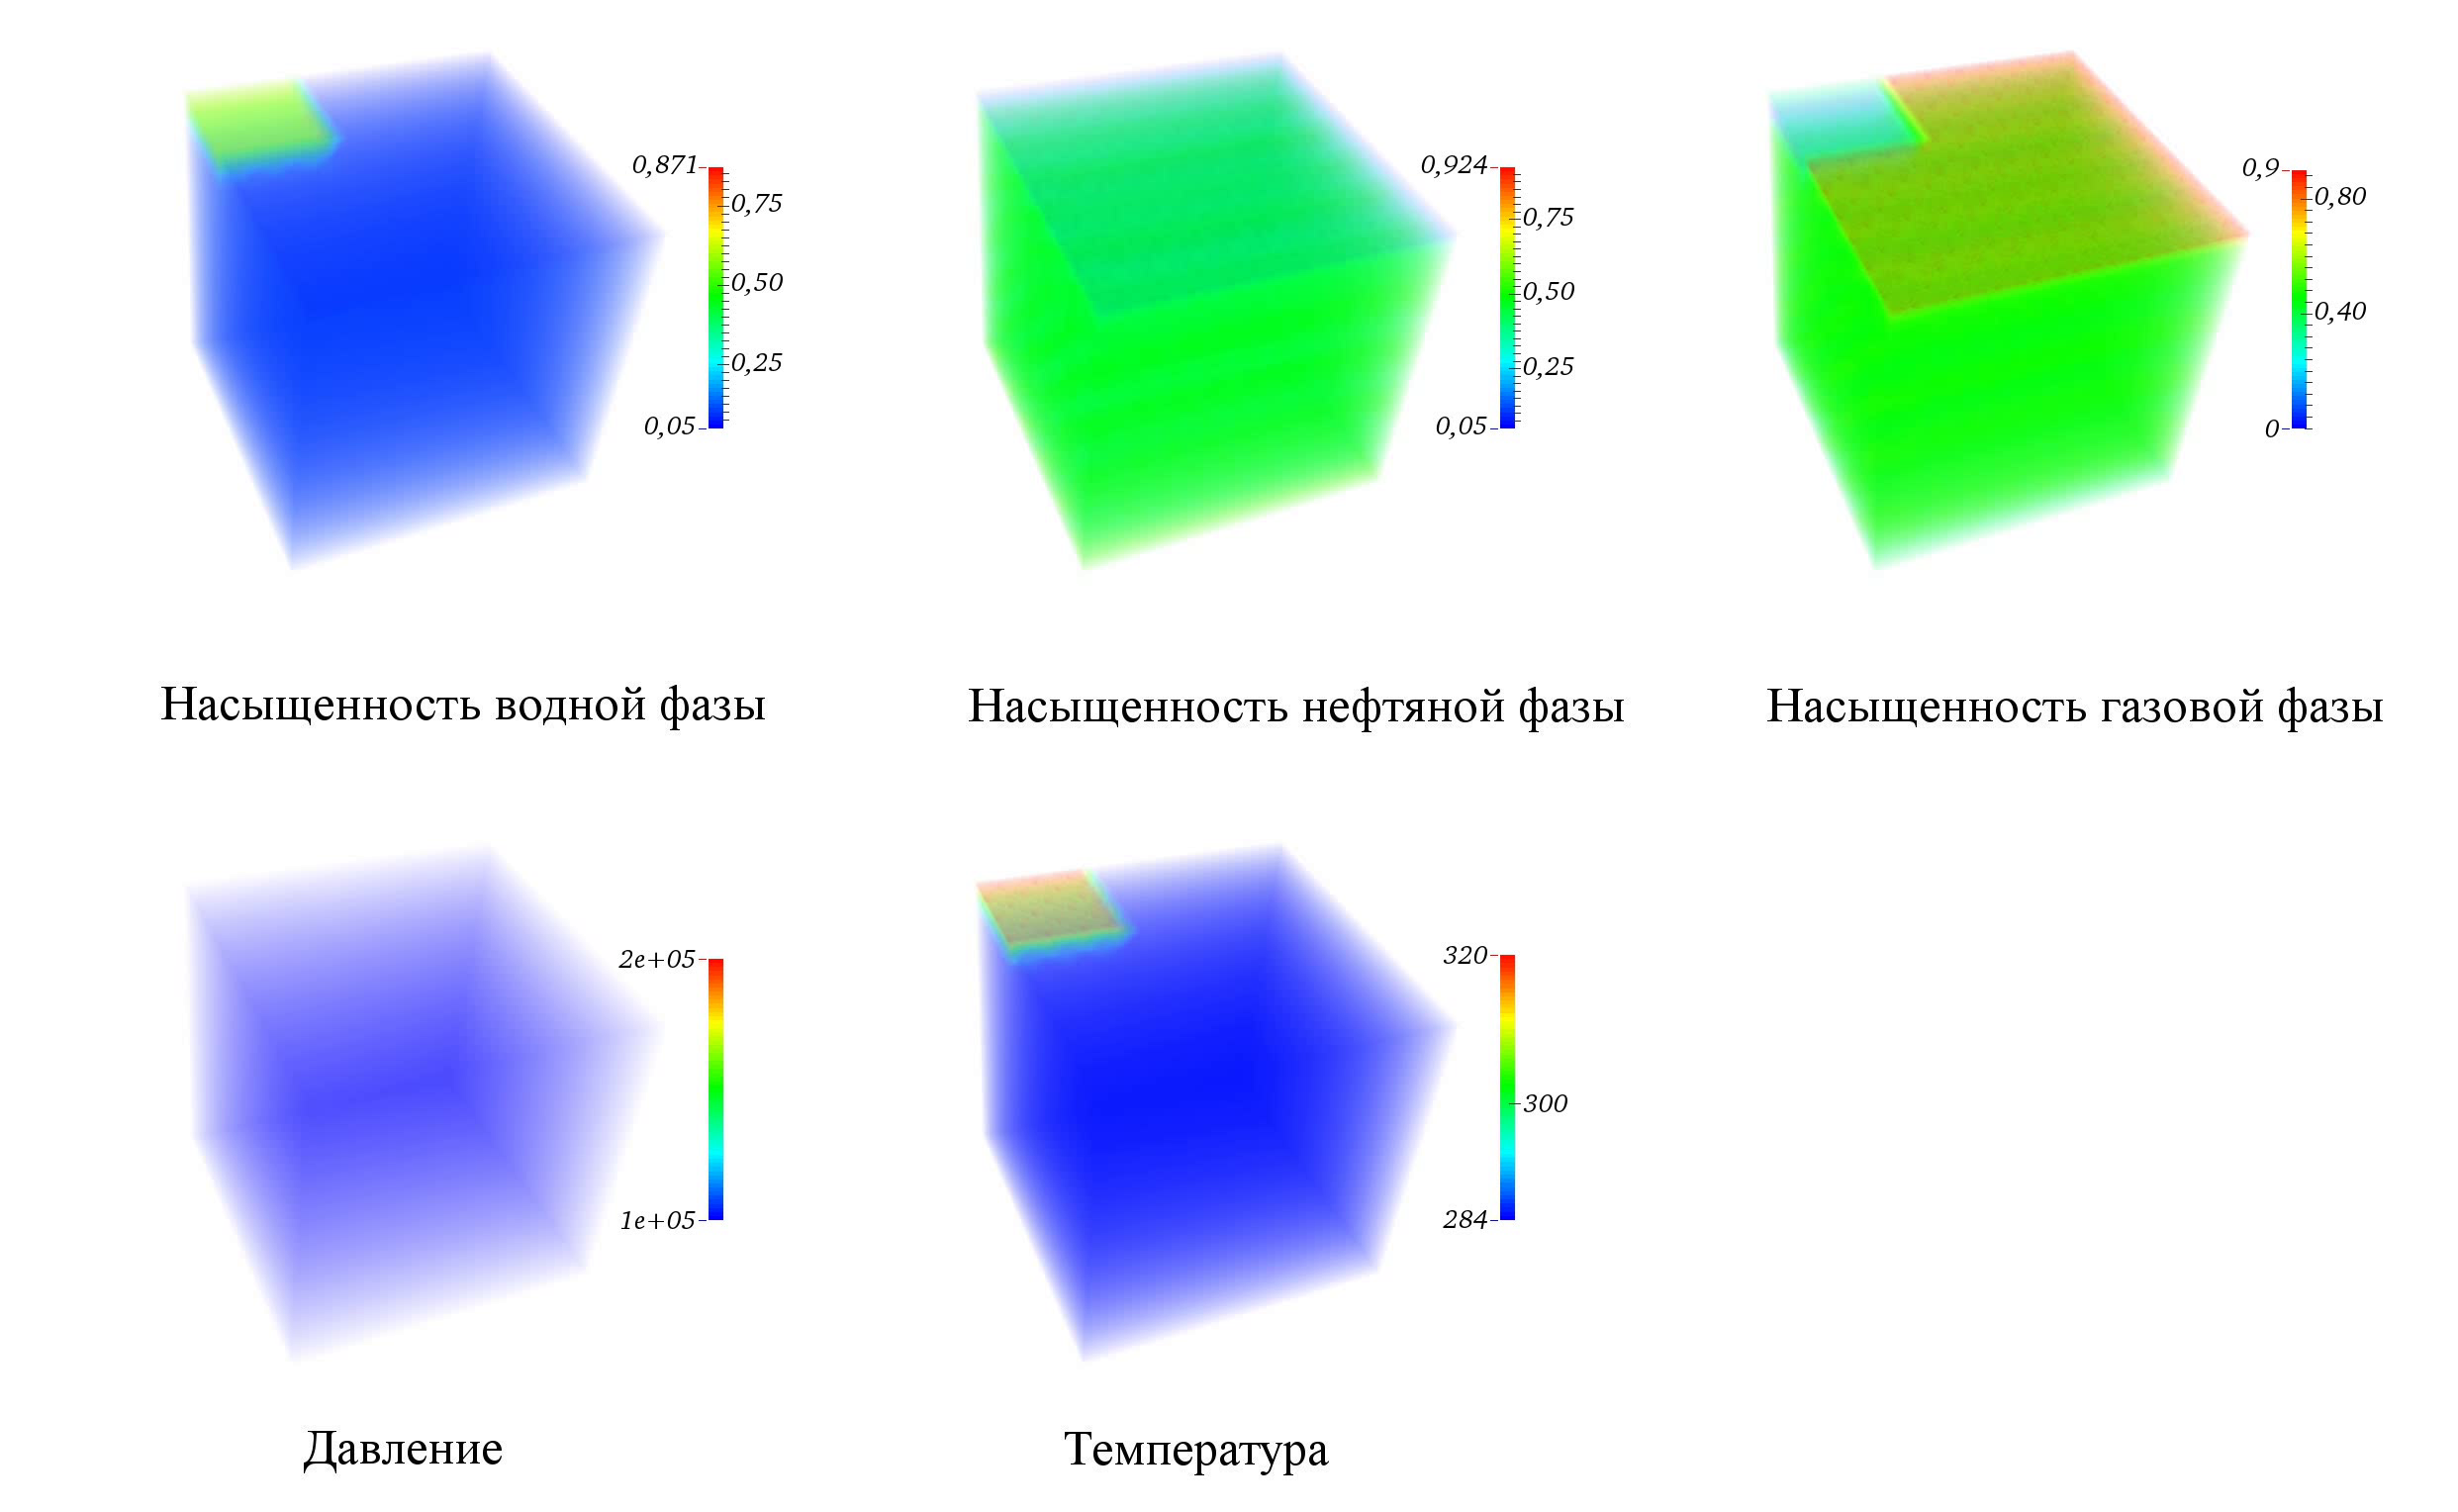
\includegraphics[width=1.0\textwidth]{video/frame.png}}{video/all_full.avi}
\end{figure}
  \end{center}
\end{frame}

